\minitoc
\section{Introduction}
Data usage control enables data owners to enforce policies for their data, 
by defining authorizations, but also obligations, which are actions to be performed before, during or after being granted access, and conditions bearing on the system and environment attributes such as the time or the system load.
Information flow control (IFC) is a security mechanism that regulates the movement of data within 
a system or network, to prevent undue dissemination of the data \cite{Denning1976}. A decentralized version called \emph{Decentralized Information Flow Control} (DIFC), was introduced by Myers and Liskov in 1997. Contrary to traditional IFC, it enables users to define policies individually or as a group without relying on a central entity. Data owners add security labels to the data directly, to indicate who is allowed to read the data \cite{Myers1997}.
While usage control and information flow control are two different technologies, they are used jointly by modern usage control systems (UCS)~\cite{Harvan2009}. Therefore, recent models~\cite{Kelbert2018, Fromm2020} tend to encompass both aspects as usage control needs to prevent dissemination in areas outside of the monitoring scope. Introducing usage control can therefore lead to unclear statements, as it is hard to distinguish whether usage control refers to classic usage control, i.e., UCON and derived models, or classic usage control with information flow control. For disambiguation, the following terminology is used
in this chapter:
  
\begin{itemize}
    \item \emph{data usage control} (UCON): refers to the policies which define the users' rights to access data, based on authorizations, obligations, and conditions;
    \item \emph{information flow control} (IFC): refers to the policies about the movement of data within the system, to monitor dissemination;
    \item \emph{usage control}: refers to both data usage control and information flow control. It is the general term, corresponding to modern usage control;
    \item \emph{a usage control system} (UCS): an entity, centralized or distributed, that is responsible for enforcing usage control.
\end{itemize}

A formal model of data usage control can help ensure that the system's security and privacy goals are achieved by providing a clear specification of the access control policies, the resources to be protected, and the roles and responsibilities of the participants in the system. While this modeling has been abundantly addressed in the state of the art in centralized settings \cite{Pretschner2011, Kelbert2013, Kelbert2014, Fromm2020}, it is still incomplete in distributed systems, considering only the distribution of the usage control system (UCS) components, but not of the other system users, notably the policy makers and the data readers \cite{Kelbert2015, Kelbert2018}.

Kelbert and Pretschner have proposed a formal model for usage control in distributed systems in 2018 \cite{Kelbert2018} that constitutes the state of the art. It focuses on the distribution of the UCS components, to enable local policy evaluation.
In this chapter, we propose to add the DIFC model \cite{Myers1997} to this state-of-the-art formalism. DIFC can be used in contexts where data are derived from several sources and all sources must agree to grant or deny access to the data \cite{Myers1997}. It further distributes the system by enabling the definition of policies on data owned by several owners. To this end, we propose the following contributions:

\begin{itemize}
    \item the definition of data usage control and information flow control policies in a distributed fashion, further enabling a better consideration of the distribution dimension; 
    \item fine-grained information flow tracking with better granularity as DIFC harnesses application-layer semantics \cite{Liu2022}, which is a known limit of the state of the art \cite{Kelbert2018};
    \item the enrichment of the state-of-the-art formalism for distributed systems \cite{Kelbert2018}, introducing novel functions and dedicated DIFC components to design and manage decentralized policy making.
\end{itemize}

The integration of DIFC is made possible by recent advances in coding practices, highlighted by Liu \emph{et al.}~\cite{Liu2022}. Past approaches to DIFC have required dedicated instrumentation efforts or developer support, which caused little adoption. Nowadays, DIFC can be leveraged by relying on application event logging, a best practice in software development used for telemetry\footnote{\cul{Telemetry is the \emph{in situ} collection of measurements or other data at remote points and their automatic transmission to receiving monitoring equipment}} and debugging \cite{Liu2022}.

The chapter is structured as follows. First, decentralized information flow control elementaries and the state of the art are provided (Section~\ref{S_DIFC}), before introducing the current modeling of usage control for distributed systems (Section ~\ref{S_data_usage_control}). We then detail the extension of the existing modeling as our contribution (Section~\ref{S_proposed_extension}), before concluding (Section~\ref{S_conclusion_formalism}).
\section{Background on decentralized information flow control}
\label{S_DIFC}

In this section, after the introduction of the DIFC model (Section \ref{ss_DIFC_model}), we detail the reasons why decentralized information flow control, while being a canonical approach to access control in systems, was not actually implemented and largely adopted (Section \ref{ss_difc_constraints}). Recent advances in software development enable the use of DIFC without additional development costs, which is explained in Section \ref{ss_advances_difc}

\subsection{DIFC model}
\label{ss_DIFC_model}
In addition to information flow control, Myers and Liskov \cite{Myers1997} proposed a decentralized version of information flow control (DIFC).
The main motivation behind DIFC is to provide a security mechanism for distributed systems. The DIFC model allows users to declassify information in a decentralized way, by delegating security to users and groups rather than a monolithic organization or entity, such as the usage control system.
In DIFC, the users in the system assign \emph{labels} to data, and then the system enforces access control policies based on these labels. DIFC labels are defined as pairs of owner-readers $p$: $\{O : R\}$, where owner $O$ allows the set of readers  $R$ to read the information on which the label is attached. The labels represent the sensitivity or confidentiality of the data and the clearance level of the users. The labels are attached to the data \mul{by} users and are propagated through the system as the information flows from one component to another. 
Myers and Liskov \cite{Myers1997} also introduce the following objects, independently of the existing information flow control modeling:

\begin{itemize}
    \item \emph{values} that are used in computations;
    \item \emph{slots} that are storage locations for values that can take different forms like variables in a code as well as a memory space in the hard drive;
    \item \emph{channels} which can be either \emph{input channels} to read data or \emph{output channels} to write data. Input channels are read-only slots that allow information to enter the system \cul{monitored by DIFC mechanisms}, while output channels are write-only slots that serve as an information sink to transmit data outside the system;
\end{itemize}

\mul{In DIFC, labels can be attached to values, but also to slots (and channels which are a particular type of slots).} 

\mul{\textbf{Operations on labels.} In DIFC, the label on a value cannot change, but a new copy of the value
can be created with a new label}. \cite{Myers1997} \mul{When this happens we say the
value is \emph{relabeled} even though only the copy has a new
label. The key to secure flow is to ensure that any relabeling is
consistent with the security policies of the original labeling. Only values can be relabeled, not slots and channels. There are two types of relabeling. \emph{Restrictions} are relabeling allowing fewer accesses than the original label. \emph{Declassifications} conversely add more readers to the label. If a label attached to a value can not change, it is possible to have \emph{multiple labels} corresponding to different owners.
}
\subsection{DIFC implementation challenges}
\label{ss_difc_constraints}
While decentralized flow control enables to make data policies whose ownership is shared by several owners, it has several shortcomings which severely limited
its adoption in real systems~\cite{Liu2022}. A major factor limiting the use of DIFC is the tremendous cost in terms of development. DIFC implementations assume that programs are modified to be able to add, remove and handle labels (Cf. Section \ref{ss_DIFC_model}).

\cul{Besides, DIFC implementations can operate at different levels of abstraction like IFC implementations, e.g., operating system level or algorithmic level. DIFC implementations relying on run-time mechanisms} (cf. Section \ref{ss_information_flow_control}) \cul{are employed at the operating system and programming language levels, which requires additional modifications at this level, making DIFC even more cumbersome} \cite{Liu2022}.

\subsection{Advances in DIFC}
\label{ss_advances_difc}
The above-mentioned limitations to DIFC adoption (cf. Section \ref{ss_difc_constraints}) have been addressed indirectly by evolving best coding practices. Indeed, applications now tend to have a security context in the form of \emph{application event logs}, for debugging, fault detection and telemetry. Events are at the root of information flow control and can be used by DIFC at the application system layer, without requiring additional development costs. Liu \emph{et al.}~\cite{Liu2022} consequently presented their solution \emph{T-DIFC}\footnote{\cul{T-DIFC stands for transparent decentralized information flow control}} to define DIFC policies based on the inspection of application logging, i.e., using the application layer. Verifying policies at the application level spares the administrator from the need for additional development.

\section{Existing usage control modeling }
\label{S_data_usage_control}

The following sections introduce the state of the art in data usage control modeling in distributed systems. First, the data usage control formalism as designed for centralized settings (Section~\ref{ss_ifc_model}, Section \ref{ss_usage_control_model}) is detailed, before the specific aspects of distribution (Section~\ref{ss_distributed_system_model}). \cul{We finally detail the rationale behind the need to improve the existing model, to meet IoT requirements regarding the connection status of the network and to integrate DIFC concepts and functions} (Section \ref{ss_motivation})

\subsection{Information flow control model}
\label{ss_ifc_model}

 An information flow control model is defined by a tuple $(\mathcal{D}, \mathcal{C}, \mathcal{E}, \mathcal{I}, \mathcal{F},\Sigma)$ \cite{Kelbert2018,Fromm2020}:
\begin{itemize}
    \item $\mathcal{D}$ are all the \emph{data} to be protected in the system. \cul{Data are the equivalent of value in DIFC modeling};
    \item $\mathcal{C}$ are all representations where the data can be stored in the system and are therefore named \emph{containers}. \cul{For example, containers can represent variables, computer memory cells or a blockchain block. Containers are the equivalent of slots in DIFC modeling};
    \item $\mathcal{E}$ are \emph{events}, e.g., method invocations or system calls, that may cause a flow of data and change the system state;
    \item $\mathcal{I}$ are the \emph{principals}, all the active entities in a system, i.e., a process or a thread;
    \item $\mathcal{F}$ is the set of all naming identifiers that are used to identify containers in a system, such as the process-id;
    \item $\Sigma$ are all the possible \emph{data flow states};
\end{itemize}

For any set $S$, $\mathcal{P}(S)$ will denote all the possible subsets of $S$. For example, if $\mathcal{E}=\{e_1,e_2\}$ is a set of events, $\mathcal{P}(\mathcal{E})  \overset{def}{=} \{\emptyset, e_1, e_2, \{e_1,e_2\}\}$ is composed of all the possible subsets of $\mathcal{E}$.  

 \emph{System runs} are modeled as a set of timed \emph{traces} $\mathcal{T}: \mathbb{N} \to \mathcal{P(\mathcal{E}))}$ that maps abstract time points $t$ to a set of events $\mathcal{E}$.

An \emph{event} $e \in \mathcal{E}$ itself is composed of a name $e$.name $ \in \mathcal{N_{E}}$ ($\mathcal{N_{E}}$ \cul{is the set of event names}) and a set of parameters $e$.p $ \in \mathcal{J_{E}} \subseteq \mathcal{P(J)}$, $\mathcal{J}$ being the set of all possible parameters. Each parameter $j \in \mathcal{J}$ is in turn defined by a name $j$.name $\in \mathcal{N_{P}}$ and a value $j$.value $\in \mathcal{V_{P}}$.

Each event has two special parameters, called ($e$.obj, $e$.actual) $\in \mathcal{J_{E}}^{2}$. $e$.obj denotes the primary object of $e$, such as a file. The parameter $e$.actual is a boolean stating if the event has already happened if true or is only intended if false\footnote{\cul{this distinction is important for information flow control, as an intended event can be blocked before the data is disseminated outside the system.}}. Besides, a parameter $e$.time $\in \mathcal{J_{E}}$ indicates the event's time of observation. Note that $e$.time \cul{ is not a special parameter, as an event may not have been observed yet if it is intended} ($e$.obj and $e$.actual are always defined).
 
We say that $e_1$ refines $e_2$ if their names are the same and if the parameters of $e_1$ are a superset of $e_2$.
An event refinement is detected using the operation \emph{refines} $\subseteq \mathcal{E} \times \mathcal{E}$:

\begin{center}
    $\forall e_1, e_2 \in \mathcal{E}: e_1~refines~e_2 \stackrel{\text {def}}{\Longleftrightarrow} e_{1}$.name = $e_{2}$.name $\land e_{1}.$p $\supseteq e_{2}.$p    
\end{center}
where $e_{1}.name$, $e_{2}.names$ are the names of the events $e_1$ and $e_2$, and $e_{1}.p$, $e_{2}.p$ are the parameters of the events $e_1$ and $e_2$. Refinement is useful to specify only relevant event parameters \cul{and exclude the parameters that are not useful for the evaluation of a given policy, or conversely to gather additional parameters, depending on the use case}.
As an example, if we consider the following events:
\begin{center}
$e_1 = (send, (obj, mail), (actual, true), (to, "user@xyz.com"))$

and $e_2 = (send, (obj, mail), (actual, true), (to, "user@xyz.com"), (from,"admin@xyz.com" ))$
\end{center}
then, we can say that $e_2$ refines $e_1$ as the parameters $e_2$.p are a superset of $e_1$.p

The \emph{traces} $\mathcal{T}$ model system runs by mapping abstract points in time $i \in \mathbb{N}$ to all system events that happened since $i-1$. Traces are formally defined as: 
\begin{center}
$\mathcal{T}: \mathbb{N} \to \mathcal{P(\mathcal{E})}$, such that $ \forall t \in \mathcal{T}, \forall i \in \mathbb{N}, i > 0, \forall e \in t(i) : i-1 < e.$time$ \leq i $ 
\end{center}
The set of all possible \emph{data flow states} $\Sigma$ is defined as $\Sigma \overset{def}{=} s \times a \times n$ where $s, a $ and $n$ are three mappings. Each state $\sigma \in \Sigma$ is defined by 
\begin{itemize}
    \item $s$ is a \emph{storage function}, $s: \mathcal{C} \to \mathcal{P}(\mathcal{D})$ \cul{returns the data stored in a container}, capturing which containers \emph{potentially} store which data;
    \item $a$ is an \emph{alias function}, $a:  \mathcal{C} \to \mathcal{P}(\mathcal{C})$ \cul{which returns the list of containers that may be updated when a given container is updated}. It captures the fact that some containers are automatically updated when others do, which is the case when containers store a copy of the same data and those data are modified. 
    \item $n$ is a naming function, $n: \mathcal{F} \to \mathcal{C}$ mapping identifiers to containers. For each state $\sigma \in \Sigma$, $\sigma$.n, $\sigma$.a and $\sigma.n$ refers to those mappings.
\end{itemize}

With the introduction of data flow states, it is now possible to extend the \emph{refines} operator to $\emph{refines}_{\Sigma}$ which describes the refinement of an event in the presence of a given state. The need for the introduction of $\emph{refines}_{\Sigma}$ is that system events always operate on containers $\mathcal{C}$, while policies may be specified in terms of data $\mathcal{D}$. We say that ($e_1,\sigma$) refines $e_2$ if either:
\begin{enumerate}
    \item both $e_1$ and $e_2$ operate on the same container and if $e_1$ \emph{refines} $e_2$;
    \item if $e_1$ operates on some container $c \in \mathcal{C}$ and $e_2$ on some data $d \in \mathcal{D}$
    within $c$ and $e_1$ \emph{refines} $e_2$ when ignoring the parameter $e$.obj.
\end{enumerate}

Therefore, the definition of ($e_1,\sigma$) \emph{refines} $e_2$ is :

    \begin{figure}[htbp]
        \begin{adjustbox}{width=\textwidth}
        \begin{minipage}{\textwidth}
        \begin{alignat*}{3}
        \forall e_1 \in \mathcal{S}, e_2 \in \mathcal{E}, \sigma \in \Sigma: \left(e_1, \sigma\right) \emph{refines}_{\Sigma} \ e_2 & \overset{\text { def }}{\Longleftrightarrow} \quad && \exists c \in \mathcal{C}: e_1 . obj=c \wedge e_2 . obj=c \wedge e_1 \emph{refines} \ e_2 \\
        & \quad && \vee \exists c \in C, d \in \mathcal{D}: e_1 . n=e_2 . n \wedge e_1 . obj=c \wedge e_2 . obj=d \\
        & \quad && \wedge d \in \sigma . s(c) \wedge e_{1 .} . p \backslash\{(obj, c)\} \supseteq e_2 . p \backslash\{(obj, d)\}
        \end{alignat*}
        \end{minipage}
        \end{adjustbox}
        \end{figure}
        
\sul{The different elements that have been introduced in this section enable us to model the information flow. However, it is also necessary to model usage control policies, i.e., how data can be used.
Besides, it is necessary to model the reaction of the system when information flow policy violations are detected, which we discuss next.}

\subsection{Modeling usage control policies with ECA rules}
\label{ss_usage_control_model}
\sul{While in the preceding section (Section} \ref{ss_ifc_model}), \sul{we introduced the model of information flow control, we now detail the modeling around data usage control policies, using ECA rules.}

\textbf{ECA rules}. Usage control policies can be translated into Event-Condition-Action rules (ECA) to facilitate their enforcement at the PEP \cite{Kumari2013}. The semantics of the ECA rules is as follows: if an event $e'$ refining the trigger Event $e$ (E) is observed at timestep $i$ and if the execution of this event would make the Condition C true, then the additional Action A may be performed at timestep $i + 1$. Actions include allowance, inhibition or delaying the event $e'$ as well as the execution of other events. 

ECA rules are expressed using four different operators with the following syntax:

\begin{center}
\begin{scriptsize}    
$ \Psi \overset{def}{=} \underline{true} | \underline{false} | \mathcal{E} $

$ \Omega \overset{def}{=} \underline{notIn}(\mathcal{D}, \mathcal{P}(\mathcal{C})) | \underline{combined}(\mathcal{D}, \mathcal{D}, \mathcal{P}(\mathcal{C})) | \underline{maxIn}(\mathcal{D,\mathbb{N},\mathcal{P}(\mathcal{C})}) $

%Can put phi on one line by spreading the margins, but matters only for the article
$\Phi \overset{def}{=} (\Phi) | \Psi | \Omega | \underline{not}(\Phi) | \Phi \underline{and} \Phi | \Phi \underline{or} \Phi | \Phi \underline{since} \Phi | \Phi \underline{before} \mathbb{N} |$
$ \underline{repmin}(\mathbb{N}, \mathbb{N}, \mathcal{E}) | \underline{repmax}(\mathbb{N}, \mathbb{N}, \mathcal{E}) | \underline{always}(\Phi) | \underline{evalExt}(\Gamma)$

$\Gamma \overset{def}{=} \Psi | \mathbb{N} | op | String | ...$
\end{scriptsize}
\end{center}

In the above syntax, $\mathcal{D}$ represents a set of data items, $\mathcal{C}$ a set of containers and $\mathcal{E}$ a set of events.
$\Gamma$ is designed to incorporate external specifications and evaluation logic. It is left unspecified, but usually leverages XPath\footnote{\cul{XPath (XML Path Language) is an expression language designed to support the query or transformation of XML documents. It enables the extraction of external specifications from XML documents.}} for this purpose \cite{Feth2012, Wuchner2012}. This part of the formalism is meant to enable generalization. Operator $\underline{evalExt}$ allows to incorporate external specification and evaluation logics, to specify conditions that refer to subject and object attributes or environmental conditions, such as time and location. $\underline{evalExt}$ as a general operator could be used for DIFC incorporation but requires additional evaluation to ensure the incorporation's correctness \cite{Kelbert2018}.

$\Omega$ defines state-based operators that constrain the data flow state, which is directly related to the place of data within the containers. Notably, $\underline{notIn}(d,\mathcal{C})$ is true if the data $d$ is not in any of the containers of $\mathcal{C}$, $\underline{maxin}(d,m,\mathcal{C})$ if $d$ is contained in at most $m$ containers of $\mathcal{C}$. In other words, $\Omega$ constrains the allowed states and by combination determines in which containers $D$ must or must not be contained. The $\underline{combined}(d_1, d_2, \mathcal{C})$ operator is true if there exists at least one container $c \in \mathcal{C}$ containing $d_1$ and $d_2$

$\Psi$ intuitively refers to the constants \underline{true} and \underline{false}, but also to events $\mathcal{E}$. \cul{For instance, an event operator} \underline{refine}\cul{($e$) where $e$ is in $\mathcal{E}$ evaluates to} \underline{true} \cul{if and only if an event refining $e$ is happening in the current timestep and the current data flow state}. Finally, $\Phi$ defines the propositional, temporal and cardinality operators. \underline{not}, \underline{and}, \underline{or} and \underline{always} are intuitive. $\alpha$ \underline{since} $\beta$ is true if $\beta$ was true at a moment earlier, i.e., during a former timestep and regardless of the current status, and $\alpha$ is true since then, or always true. $\alpha$ \underline{before} $j \in \mathbb{N}$ is true if $\alpha$ was true exactly $j$ timesteps ago. 
\underline{repmin} and \underline{repmax} correspond respectively to an event appearing at least or at most $n$ times during the $j$ last timesteps.

\subsection{Existing usage control model for distributed systems}
\label{ss_distributed_system_model}

\cul{We now introduce the distribution aspects of the state-of-the-art formalism on data usage control. These aspects are threefold. First, the selective distribution of the UCS components. Second, the separation of the whole distributed system into individual systems, that can be merged into sets of individual systems. Finally, the introduction of functions to identify the relevant system sets to evaluate usage control policies.} 

\textbf{Local PDP/PIP components.} The first step to the distribution is the introduction of local PDP/PIP couples (cf. Section \ref{ss_ucon_architecture}), to take policy decisions locally \cite{Kelbert2018}. Distributing these couples however requires handling the communication between the distributed instances, which would otherwise create a significant overhead. In the worst-case scenario, all instances of PDP/PIP couples must share their local environment with all the other instances. The communication cost increases exponentially with the number of couples. Optimization effort is compulsory to make the distributed policy evaluation viable. 

\textbf{Individual systems.} To optimize policy enforcement in distributed systems, it is necessary to identify the relevant set of systems where a given policy must be enforced. This is useful as 1) it avoids monitoring the whole network for every policy; 2) it reduces the network exchanges between the different PDP instances. 

\emph{Individual systems} $\mathcal{Y}$ constitute the autonomous parts of the distributed system \cite{Kelbert2018}. A \emph{system} is a non-empty set of individual systems whose PEPs share the same PDP/PIP couple. Each individual system $y \in \mathcal{Y}$ has its own events $\mathcal{E}_{y}$, its own containers $\mathcal{C}_{y}$, its own set of identifiers $\mathcal{F}_{y}$, its own system runs $\mathcal{T}_{y}$, and its own possible data flow states $\Sigma_{y}$. Each event $e$ is required to carry a parameter $e$.sys with sys $\in \mathcal{N}$ ($\mathcal{N}$ is a set of names) \cul{to identify the system in which it is happening}. In practice, individual systems run in parallel and have independent traces and flow states. 
 For policy enforcement, the reasoning must be done on sets of individual systems, called \emph{sets of systems} $Y \subseteq \mathcal{Y}$ or on the whole distributed system. Sets of systems also have : 
 \begin{enumerate}
 \item a set of events defined as the union of individual system's events: $\mathcal{E}_Y \overset{def}{=} \cup_{y \in Y} \ \mathcal{E}_{y} $;
 \item a set of containers $\mathcal{C}_Y \overset{def}{=} \cup_{y \in Y} \ \mathcal{C}_{y} $;
 \item a set of identifiers $\mathcal{I}_Y \overset{def}{=} \cup_{y \in Y} \ \mathcal{I}_{y} $; 
 \item a set of possible system runs (modeled by traces) $\mathcal{T}_Y : \mathbb{N} \to \mathcal{P}(\mathcal{E}_{Y})$. At the difference of the other parameters, traces can not be formed as the union of the possible system runs of the individual systems composing the set of systems. 
 \end{enumerate}
\textbf{Relating individual systems with system sets.}
From individual system traces, it is possible to define the combined traces of systems \cite{Kelbert2018}. Let $\prod$ be the Cartesian product of sets. We can define $\tau \in \prod_{y \in \mathcal{Y}}\mathcal{T}_{y} $ as a \cul{set} of traces of all individual systems. $t_{y}^{\tau} \in \mathcal{T}_{y}$ refers to the trace of the system $y \in \mathcal{Y}$ while $\sigma_{t_y}$ refers to the corresponding data flow state. $t_{Y}^{\tau} \in \ \mathcal{T}_{Y}$ is defined as the combined traces of systems $Y \subseteq \mathcal{Y}$. For each timestep $i \in \mathbb{N}$, the set of events observed in $Y$ is the union of the events in all individual systems $y \in Y$, such that: 
\begin{center}
$\forall Y \subseteq \mathcal{Y}, i \in \mathbb{N}, \tau \in \prod_{y \in \mathcal{Y}}\mathcal{T}_{y}, t_{Y}^{\tau} \in \mathcal{T}_{Y} : t_{Y}^{\tau}(i) \overset{def}{=} \bigcup_{y \in Y}t_{y}^{\tau}(i)$
\end{center}
This corresponds to what a centralized PDP would observe.
Analogously, we combine the data flow states of individual systems to form a global data flow state $\sigma_{t_{Y}^{\tau}}$, representing what a central PIP would observe. For convenience, $\forall i \in \mathbb{N}$ a given timestep, $\sigma_{t_{y}^{\tau}}(i)$ will be noted $\sigma_{t_{y}^{\tau}}^{i}$ in the following. $\sigma_{t_{y}^{\tau}}$  is constructed by unifying the mappings of the individual systems’ storage, alias, and naming functions:


\begin{center}
\begin{small}
    $\forall Y \in \mathcal{Y}, i \in \mathbb{N}, \tau \in \prod_{y \in \mathcal{Y}}\mathcal{T}_{y}, y \in Y, t_{Y}^{\tau} \in \mathcal{T}_{Y}, t_{y}^{\tau} \in \mathcal{T}_{y}, \sigma_{t_{Y}^{\tau}}^{i} \in \Sigma_{Y}, \sigma_{t_{y}^{\tau}}^{i} \in \Sigma_{y}, c \in \mathcal{C}_{y}, j \in \mathcal{I}_{y}$:
\end{small}    
$\Sigma_{Y} \subseteq \Sigma : (\mathcal{C}_{Y} \to \mathcal{P}(\mathcal{D})) \times (\mathcal{C}_{Y} \to \mathcal{P}_{Y}) \times (\mathcal{I}_{Y} \to \mathcal{C}_{Y})$
\end{center}
which leads to the definition of $\sigma_{t_{Y}^{\tau}}^{i}.s(c)$ such that: 
\begin{center}
    $\sigma_{t_{Y}^{\tau}}^{i}.s(c) \overset{def}{=} \sigma_{t_{y}^{\tau}}^{i} \wedge \sigma_{t_{Y}^{\tau}}^{i}.a(c) \overset{def}{=} \sigma_{t_{y}^{\tau}}^{i}.a(c) \wedge \sigma_{t_{Y}^{\tau}}^{i}.n(j) \overset{def}{=} \sigma_{t_{y}^{\tau}}^{i}.n(j)$
\end{center}

To recapitulate, $t_{Y}^{\tau}$ and $\sigma_{t_{y}^{\tau}}^{i}$ of set of systems $Y$ are the reflection of the trace ($t_{Y}^{\tau}$) and the state ($\sigma_{t_{y}^{\tau}}^{i}$) of $Y$.

\textbf{Identification functions.} To avoid unnecessary communication, functions are needed to identify the relevant systems for evaluating the policy $p$. First, the three following auxiliary functions are defined \cite{Kelbert2018}:

\begin{enumerate}
    \item \emph{knowC}: $\mathcal{P}(\mathcal{C}) \to \mathcal{P}(\mathcal{Y})$. Given a set of containers $\mathcal{C}$, \emph{knowC} returns the set of systems in which one of the containers $c \in \mathcal{C}$ resides. The formal definition of \emph{knowC} is: $\forall C \in \mathcal{C}: \emph{knowC}(C) \overset{def}{=} \{y \in \mathcal{Y} | \mathcal{C}_{y} \cap C \neq \emptyset\}$;
    \item \emph{knowD}: $\mathcal{P}(\mathcal{D}) \times \mathbb{N} \times \prod \mathcal{T} \to \mathcal{P}(\mathcal{Y})$. Given a set of data items $\mathcal{D}$, a point in time $t \in \mathbb{N}$ and a tuple of concurrently executing traces $\mathcal{T}$, \emph{knowD} relies on the systems' information flow to return the set of systems where there are one or more containers store at least one of the data items $d \in \mathcal{D}$:
    
    $\forall D \subseteq \mathcal{D}, i \in \mathbb{N}, \tau \in \prod_{y \in \mathcal{Y}} \mathcal{T}_{y}: $ \emph{knowD}$(D,i,\tau) \overset{def}{=} \{y \in \mathcal{Y} | \exists c \in \mathcal{C}_{y}, t_{y}^{\tau} \in \mathcal{T}_{y}, \sigma_{t_{y}^{\tau}}^{i} \in \Sigma_{y}: D \cap \sigma_{t_{y}^{\tau}}^{i}.s(c) \neq \emptyset \} $
    
    \emph{knowD} is parameterized in time \cul{and requires traces as input}, as data are continuously propagated across systems;
    \item \emph{happens}: $\mathcal{E} \times \mathbb{N} \times \prod \mathcal{T} \to \mathcal{P}(\mathcal{Y})$. Given an event $e \in \mathcal{E}$, a point in time, and a tuple of concurrently executing traces, \emph{happens} returns the set of systems where any event refining $e$ happens.
    $\forall e \in \mathcal{E}, i \in \mathbb{N}, \tau \in \prod_{y \in \mathcal{Y}} \mathcal{T}_{y}:$ \emph{happens}$(e,i,\tau) \overset{def}{=} \{y \in \mathcal{Y} | \exists t_{y}^{\tau} \in \mathcal{T}_{y}, e' \in t_{y}^{\tau}(i), \sigma_{t_{y}^{\tau}}^{i} \in \Sigma_{y}: (e', \sigma_{t_{y}^{\tau}}^{i}) \  \emph{refines}_{\Sigma} \ e\} $
\end{enumerate}
   \mul{Using these three auxiliary functions, the \emph{relevant} function is composed so as to detect individual systems potentially interesting for the evaluation of policies}. For a policy $p$, \emph{relevant}: $\Phi \times \mathbb{N} \times \prod \mathcal{T}$ identifies the set of systems that may contribute to the evaluation of conditions $\varphi_{p} \in \Phi$ at a given timestep $i \in \mathbb{N}$ and given a set of concurrently executing traces $\tau \in \prod_{y \in \mathcal{Y}} \mathcal{T}_{y}$.
   
%    \emph{relevant} is defined using the operators $\Psi,\ \Omega,\ \Phi \ and \ \Gamma$ (cf. Figure \ref{F_relevant}).

% \begin{figure}[htbp]
%     \begin{adjustbox}{width=\textwidth}
%     \begin{minipage}{\textwidth}
%     \begin{align*}
%     & \forall \varphi \in \Phi, i \in \mathbb{N}, \tau \in \prod_{y \in \mathcal{Y}} \mathcal{T}_y: \text{relevant}(\varphi, i, \tau) \stackrel{\text { def }}{=} \{y \in Y \mid \\
%     & \left(\left(\varphi=\underline{true} \ \vee \varphi =\underline{false}\right) \Longrightarrow Y= \emptyset \right) \ \ \textbf{(1)} \\
%     & \vee \exists e \in \mathcal{E} \cdot(\varphi=e \Longrightarrow Y=\text { happens }(e, i, \tau)) \ \textbf{(2)} \\
%     & \vee \exists d \in \mathcal{D}, m \in \mathbb{N}, C \subseteq \mathcal{C} \cdot((\varphi=\underline{notIn}(d, C) \vee \varphi=\underline{maxin}(d, m, C)) \Longrightarrow \quad Y= \operatorname{knowD}(\{d\}, i, \tau) \cap \text {knowC}(C)) \ \textbf{(3)} \\
%     & \vee \exists d_1, d_2 \in \mathcal{D}, C \subseteq \mathcal{C} \cdot\left(\varphi=\underline{combined}\left(d_1, d_2, C\right) \Rightarrow Y=\operatorname{knowD}\left(\left\{d_1\right\}, i, \tau\right) \cap \text { knowD }\left(\left\{d_2\right\}, i, \tau\right) \cap\right. \text {knowC}(C)) \ \textbf{(4)} \\
%     & \vee \exists \alpha \in \Phi \cdot(\varphi=\underline{not}(\alpha) \Longrightarrow Y=\text{relevant}(\alpha, i, \tau)) \ \textbf{(5)} \\
%     & \vee \exists \alpha, \beta \in \Phi \cdot((\varphi=\alpha \ \underline{and} \  \beta \vee \varphi=\alpha \ \underline{or} \ \beta) \Rightarrow \quad Y=\text{relevant}(\alpha, i, \tau) \cup \text{relevant}(\beta, i, \tau)) \ \textbf{(6)} \\
%     & \vee \exists a, \beta \in \Phi \cdot(\varphi=\alpha \ \underline{since} \ \beta \Rightarrow \quad Y=\bigcup_{j=0}^i(\text{relevant}(\alpha, j, \tau) \cup \text{relevant}(\beta, j, \tau))) \ \textbf{(7)} \\
%     & \vee \exists \alpha \in \Phi, j \in \mathbb{N} \cdot(\varphi=\alpha \ \underline{before} \ j \Rightarrow \quad Y=\text{relevant}(\alpha, i-j, \tau)) \ \textbf{(8)} \\
%     & \vee \exists j, m \in \mathbb{N}, e \in \mathcal{E} \cdot(\varphi=\underline{repmin}(j, m, e) \Longrightarrow \quad Y=\bigcup_{k=0}^{\min (i, j)-1} \text{happens(e, } i-k, \tau))\} \ \textbf{(9)}
%     \end{align*}
%     \end{minipage}
%     \end{adjustbox}
%     \caption{Definition of the function \emph{relevant} to identify systems of interest to evaluate a policy}
%     \label{F_relevant}
%     \end{figure}
    

\subsection{Rationale for extending the existing model}
\label{ss_motivation}

Distributed systems are computer systems composed of multiple independent components, such as processors, storage devices, and communication channels, that cooperate to perform a unified task. Their purpose is to provide high performance, scalability, fault tolerance, and transparency to the users. They are consequently used in several fields including the Internet of Things (IoT), Cloud computing and peer-to-peer networks.

The current state-of-the-art formalism for usage control in distributed systems of Kelbert and Pretschner~\cite{Kelbert2018} (cf. Section~\ref{ss_distributed_system_model}) indeed considers the distribution of the UCS components, notably the PDP/PIP couple. \mul{However, the dimension of user-side distribution is important, where groups of data owners define possibly conflicting policies for access. We propose to use the DIFC to define these group policies.
In general, data usage control in distributed systems is a recent field of research, and actual challenges that must be addressed are not clearly identified nor formalized} \cite{Gil2023}. 

Kelbert and Pretschner~\cite{Kelbert2018} mention DIFC in the related work, claiming that 1) data usage control policies can express similar constraints than DIFC; 2)~DIFC mechanisms can be integrated via the  \underline{evalExt} operator. While the former affirmation is partly true regarding the constraints in the policies, data usage control policies do not consider the owner-side distribution of the data, and ignore the architectural consequences for the UCS. For the second affirmation, the evaluation of external specification is indeed considered, but the \underline{evalExt} operator requires additional analyses when a concrete framework realizing \underline{evalExt} is implemented as stated by Kelbert and Pretschner \cite{Kelbert2018}
These limitations, the need to consider distribution as a whole and the recent advancements in DIFC enabling its practical use justify the integration of DIFC in distributed usage control modeling.

\mul{Besides, individual systems as defined in Section} \ref{ss_distributed_system_model} \mul{may be disconnected from the network at a given timestep} $i \in \mathbb{N}$. \mul{This is particularly true in the Internet of Things networks, as devices can be intermittent, on battery, or unreliable. The formalism must be able to take into account the possibility that a data}$d$ \mul{is present in a container, but that the system where the container is located can not be reached at a given timestep.} 

To sum up, the extension of the existing model is justified by:
\begin{enumerate}
    \item the need for users to define policies jointly in a decentralized manner. This requires the introduction of DIFC in the existing formalism, as the $\underline{evalExt}$ operator is too generic to ensure the incorporation's correctness; 
    \item the need to consider the connection status of individual systems.
\end{enumerate}
In the following Section \ref{S_proposed_extension}, we introduce auxiliary functions and dedicated components to evaluate DIFC policies \cul{in addition to} data usage control policies. This results in different functions, where the focus is on detecting conflicts between labels. \mul{Additionally, we define functions to monitor the status of a system and determine if data and containers are currently accessible}


\section{Proposed extension}
\label{S_proposed_extension}

We propose the introduction of DIFC to the existing state-of-the-art formalism for distributed data usage control. This results in new formal definitions, and new components in the usage control architecture. 
%After the motivation for using DIFC, 
In this section, an illustrative scenario is provided first to highlight the need for DIFC, before the actual details of the contribution.

\subsection{Illustrative scenario}
\label{ss_illustrative_scenario_difc}
  The illustrative scenario is again around car sharing as introduced in Section \ref{ss_illustrative_scenario}, but with a significative difference as occupants can now be in the car. They share the same geolocation data but have different privacy needs.

In this scenario, \emph{car owners} put their cars on a rental market, and \emph{car renters} pay to rent the cars. The car renter may not be alone in the car. Therefore, \emph{occupants} are also considered. \rul{The car renter $car_{rent}$, the car owner $car_{own}$ and the $i$ occupants $\mathcal{O} = \{occ_1,...,occ_i\}$ interact with the car sharing service using a \emph{mobile app}, considered trusted.} Both the car renter and the car occupants share the \emph{same geolocation data}, i.e., the location of the car. However, they may have different privacy needs, and the usage control policy should be defined by every one of them, with the most restrictive policy being applied. \mul{For instance, an occupant $p$ authorizes the car owner $c_{own}$ to monitor the car, and the car renter $c_r$ authorizes the car owner $c_{own}$ as well as third-party responsible for advertising third-parties $adv$. If $c_{own}$ logically can access the data, should $adv$ be allowed to access the data as well?  This is precisely what DIFC is designed for, as it enables users to define policies as a group by applying labels to data, without requiring a central authority.
This scenario is represented in Figure} \ref{F_DIFC_car_pooling}.

\begin{figure}[t]
\centering
 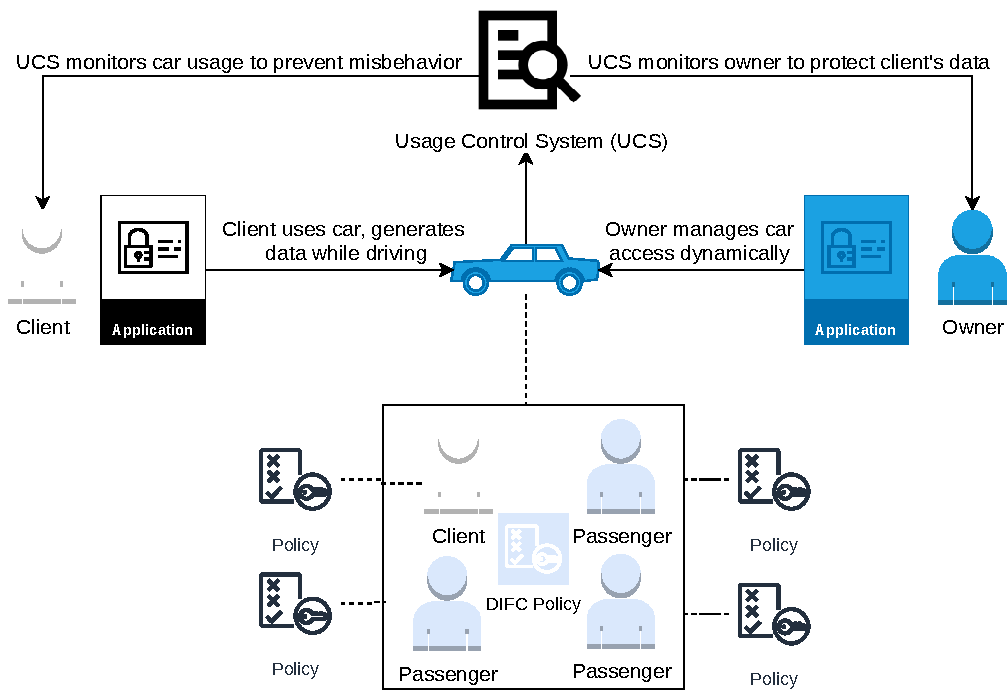
\includegraphics[width=\textwidth]{Images/framework_IFIP_alt.pdf}
\caption{Car sharing scenario and policies by car renter and occupants}
\label{F_DIFC_car_pooling}

\end{figure}
\subsection{Additional functions for DIFC and network status aspects}
\cul{As DIFC is only mentioned as an external specification in the state of the art}, DIFC objects, namely values, slots, channels and labels are not formalized in usage control models \emph{per se}. However, data $d \in \mathcal{D}$ can be regarded as DIFC values. Similarly, as containers hold the data, they can be considered as slots as defined in the DIFC specification \cul{and have labels attached to them}. A set of labels is noted $\mathcal{L}$, and can be composed of labels on any of the three DIFC objects that may be labeled, i.e., data, slots, and values. For convenience, we keep track of the objects associated with a label, such that $l.objects$ returns the list of data, slots or values associated with the label $l$. 

Having different labels, data and containers may have conflicting policies. Detecting conflicts is crucial to enforce information flow policies, as a decision must be taken to prioritize either the container labeling or the data labeling. Detecting the conflicts requires additional functions, to fetch the labels associated to containers and data, which are defined here as part of the contribution:
\begin{itemize}
    \item[] (1) \emph{labelC}: $\mathcal{P}(\mathcal{C}) \to \mathcal{P}(\mathcal{L})$. Given a set of containers, returns the labels associated with the containers: $\forall c \in \mathcal{C}$, \emph{labelC}$(c) \overset{def}{=} \{ l \in \mathcal{L} \ | c \in l.objects \} $; 
    \item[] (2) \emph{labelD}: $\mathcal{P}(\mathcal{D}) \to \mathcal{P}(\mathcal{L})$.
    Given a set of data, returns the labels associated with the data items: $ \forall d \in \mathcal{D}$, \emph{labelD}$(d) \overset{def}{=} \{ l \in \mathcal{L} \ | d \in l.objects \} $
    \item[] (3) \emph{conflict}: $\mathcal{P}(\mathcal{C}) \times \mathcal{P}(\mathcal{D}) \to \mathcal{P}(\mathcal{Y}) $. Given a set of containers $\mathcal{C}$ and data $\mathcal{D}$, returns the set of systems where there is a difference between the label associated with a container and the label of one of their known data. This function relies on \emph{knowD} (cf. Section \ref{ss_distributed_system_model}) to identify the containers $C$ knowing $d$ in the first place, then, by comparing the labels of all $c \in C$ with the labels of $d$ in $\mathcal{D}$:
    $ \forall c \in \mathcal{C}, \forall d \in \mathcal{D}
    $, \emph{conflict}$(c,d) \overset{def}{=} \{ y \in \mathcal{Y} | \exists (c,d) :$ \emph{labelC}$(c) \neq$ \emph{labelD}$(d) \}$;
\end{itemize}

The \emph{conflict} function, based on the \emph{labelC} and \emph{labelD} auxiliary functions, is dedicated to detecting individual systems $\mathcal{Y}$ where there is a conflict between the data label and the label of the container holding the data. These systems are of interest because this situation requires deciding which label should be prioritized, e.g., by considering the label representing the most restrictive policy.

\rul{In the car sharing scenario, a car owner $car_{own}$ is allowed to access the data container in its car $c_{car}$, but may not have access to the geolocation of the car $d_{GPS}$ stored in $c_{car}$. The car renter $car_{rent}$ or one of the car occupants $\mathcal{O}$ may apply labels to $d_{GPS}$ that may prevent the $car_{rent}$ from reading $d_{GPS}$. Detecting a conflict between the label $l_{c_{car}}$ applied to the container $c_{car}$ and the label $l_{d_{GPS}}$ applied to the data $d_{GPS}$ enables to block the dissemination to $car_{own}$. In that case, the security policy is to consider that the data label has priority over the container label. This policy is defined by the system administrator, and could be different, e.g., deny access in case of conflict is detected which would have the same result in this example.}

\textbf{Functions for network status.} Distributed systems are used in a diversity of networks, including the Internet of Things and peer-to-peer networks. These networks are inherently dynamic, with devices and peers connecting and disconnecting very frequently. Besides, the network may be intermittent or unreliable. For proper policy evaluation, it is consequently required to determine whether an individual system or a set of systems $\mathcal{Y}$ are currently connected to a system. \mul{More accurately, an individual (or a set of) system is considered disconnected if it can not be reached by the usage control system. The main concern in our case is the possibility to evaluate policies, and it avoids introducing more intricate notions, like relative disconnection between two individual systems}. By extension, it makes it possible to identify the subset of systems $\mathcal{Y}$ where a container $\mathcal{C}$ resides and that is connected to the distributed network. This leads to the definition of the following functions:

\begin{enumerate}
    \item[(1)] \emph{connected} : $\mathcal{Y} \times \mathbb{N} \times \prod \mathcal{T} \to \mathcal{P(Y)}$. Given a set of individual systems $\mathcal{Y}$, a point in time $i \in \mathbb{N}$ and a tuple of traces, return the subset of individual systems that are reachable in the network at this point in time. \mul{Traces are needed because the connection status depends on the timesteps considered}. An individual system is considered connected if there is no disconnection $e_{disconnect}$ in the traces, i.e., an event whose name $e$.name = disconnect. \emph{connected} is defined as: 
    \begin{center}
     $\forall y \in \mathcal{Y}, i \in \mathbb{N},  \tau \in \prod_{y \in \mathcal{Y}} \mathcal{T}_{y}$, \emph{connected}$(y,i,\tau)\overset{def}{=} \{ y \in \mathcal{Y} \ | \ \forall e \in  t_{y}^{\tau}(i), \ $e$.name \neq disconnect\}$  
    \end{center}

    \item[(2)] \emph{availableC} : $\mathcal{P(C) } \times \mathbb{N} \times \prod \mathcal{T} \to \mathcal{P(Y})  $. Given a set of containers, a point in time and a tuple of concurrently executing traces $\mathcal{T}$, \emph{availableC} returns the set of currently reachable systems in which one of the containers $c \in \mathcal{C}$ resides. The formal definition of \emph{availableC} is:
    \begin{center}
    $\forall C \in \mathcal{C}, i \in \mathbb{N},  \tau \in \prod_{y \in \mathcal{Y}} \mathcal{T}_{y}: \emph{availableC}(C) \overset{def}{=} \{y \in \mathcal{Y} \ | \ \mathcal{C}_{y} \cap C \neq \emptyset\ \wedge$ \emph{connected}$(y,i,\tau) \cap $\emph{knowC}$(C) \neq \emptyset\} $;
    \end{center}
    
    \item[(3)] \emph{availableD} : $\mathcal{P}(\mathcal{D}) \times \mathbb{N} \times \prod \mathcal{T} \to \mathcal{P}(\mathcal{Y})$. Given a set of data items $\mathcal{D}$, a point in time $ t \in \mathbb{N}$ and a tuple of concurrently executing traces $\mathcal{T}$, \emph{availableD} returns the set of currently reachable systems where one or more containers are storing at least one of the data items $d \in \mathcal{D}$. \emph{availableD} is formally defined as follows:
    \begin{center}
      $\forall D \subseteq \mathcal{D}, i \in \mathbb{N}, \tau \in \prod_{y \in \mathcal{Y}} \mathcal{T}_{y}: $ \emph{availableD}$(D,i,\tau) \overset{def}{=} \{y \in \mathcal{Y} \ | \ \exists c \in \mathcal{C}_{y}, t_{y}^{\tau} \in \mathcal{T}_{y}, \sigma_{t_{y}^{\tau}}^{i} \in \Sigma_{y}: D  \cap \sigma_{t_{y}^{\tau}}^{i}.s(c)  \neq \emptyset \ \wedge$ \emph{connected}$(y,i,\tau) \cap$\emph{knowD}$(D,i,\tau) \neq \emptyset \}$
     \end{center}
\end{enumerate}

\rul{As the cars are moving objects, the need to manage connection status is paramount in the car sharing scenario. First, a car may be disconnected temporarily from the network, e.g., driving through a tunnel, which is detected by the \emph{connected} function. As a consequence, if the location of the car $d_{GPS}$ is stored only in the car \emph{via} a data container $c_{car}$ in the car, it becomes unavailable to the car owner $car_{own}$, who should be notified. This is reflected by both \emph{availableC} and \emph{availableD}, for respectively the container $c_{car}$ and the data $d_{GPS}$.}

\sul{In this section, we introduced several formal functions to handle DIFC labels (\emph{labelC} and \emph{labelD}) and detect conflicts between the data and their containers (\emph{conflict}). Additionally, we introduced functions to handle the status of the network, detecting if a set of individual systems is connected or not (\emph{connected}), and consequently if a container can be accessed and data fetched depending on the system's state. In the next section, we introduce the new components needed in the usage control system architecture to handle DIFC aspects, as part of our contribution.}

\subsection{Integrating DIFC components in the usage control system}
\label{ss_architectural_integration_of_difc}
Distributing the system requires the introduction of several components for the UCS to handle cross-system communication, information flow tracking and policy deployment. In addition to the existing UCS components in centralized settings (cf. Section \ref{ss_ucon_architecture}), the usage control system has the following components:
\begin{itemize}
    \item The \emph{Distribution Management Point} (DMP) organizes the information flow between systems and the policy propagation while relying on a distributed database to coordinate the policy decisions,
  \item the \emph{PDP server} provides the interface so that PEPs can request data usage control decisions.
 \item The \emph{PIP Server} provides the interface to fetch environment attributes from the PIPs.
  \item The \emph{DMP Server} allows communication with remote DMPs. 
 \item the \emph{Context Handler} orders and processes requests sent to the servers, 
notably to avoid event reordering and race conditions. The architecture is represented in Figure \ref{F_Kelbert_architecture_DIFC_enhanced};
\item The \emph{communication manager} manages all external communication 
and runs servers to show the components' functionalities to the outside. It is not a component itself and is composed of the Context Handler, PDP server, PIP server and DMP server. 
\end{itemize}
% Distributing the system requires the introduction of several components for the UCS to handle cross-system communication, information flow tracking and policy deployment. The \emph{Distribution Management Point} (DMP) organizes the information flow between systems and the policy propagation while relying on a distributed database to coordinate the policy decisions.
%  The \emph{communication manager} (included in the controller) manages all external communication 
% and runs servers to show the components' functionalities to the outside. In particular, the \emph{PDP server} provides the interface so that PEPs can request data usage control decisions.
% The \emph{PIP Server} provides the interface to fetch environment attributes from the PIPs. The \emph{DMP Server} allows communication with remote DMPs. Finally, the \emph{Context Handler} orders and processes requests sent to the servers, 
% notably to avoid event reordering and race conditions. The architecture is represented in Figure \ref{F_Kelbert_architecture_DIFC_enhanced}. 



\textbf{Additional components for DIFC processing.} Decentralized information flow control is often processed using a dedicated instance, called the DIFC platform \cite{Schultz2013} or DIFC center \cite{Lu2022}. There are different ways to process DIFC tasks: either use already existing components, e.g., the PDP, or introduce new dedicated components to manage DIFC aspects. Since DIFC policies differ from usage control policies, it is better to introduce dedicated components to handle DIFC aspects.

For distribution purposes, DIFC platform components are added as a novelty to the existing architecture \cite{Lu2022}, and interact only with the DMP to distribute the policies to other individual systems $\mathcal{Y}$ or system set $Y$. The DIFC platform is responsible for pre-processing (DPP), privilege extraction (PP) and data labeling (DLP). Each operation has a dedicated component, as depicted in Figure~\ref{F_Kelbert_architecture_DIFC_enhanced}:
\begin{itemize}
    \item the \emph{Data Labeling Point} (DLP) is responsible for labeling data, slots and channels;
    \item the \emph{Privilege Point} (PP) is responsible for privilege extraction, converting labels into actual access rights;
    \item the \emph{Data Pre-processing Point} (DPP) routes the data to other components of the DIFC platform. If the data is unlabeled, the data are sent to the DLP. Conversely, labeled data are sent to PP for privilege extraction (cf. Section \ref{ss_DIFC_model}).
\end{itemize}


\textbf{Existing interfaces.}
Interfaces are associated with the components to provide several methods for usage control.
The PDP server provides two interfaces \texttt{IPmp2Pdp} and \texttt{IPep2Pdp}, providing methods to deploy or retrieve policies,  
to signal system events and to await policy decisions.
The PDP uses interface \texttt{IPdp2Pip} to evaluate state-based operators, retrieve all data stored in a  
container $\mathcal{C}$, and signal system events associated with information flow. The PMP uses interface \texttt{IPmp2Pip} to inform the PIP about initial data
representations. Interface \texttt{IDmp2Pip} is used by the DMP if there are cross-system data flows.
The DMP provides interface \texttt{IDmp2Pmp}, which is used by the local DMP to deploy policies and to retrieve currently
deployed policies. The DMP additionally provides four interfaces:

\begin{enumerate}
    \item \texttt{IPip2Dmp} allows the PIP to inform the DMP about data flows to the remote socket
    containers;
    \item \texttt{IPdp2Dmp} enables the coordination of policy decisions across PDPs. This includes methods to notify
    that an operator’s state has changed, to query whether the state of some operator has changed at remote PDPs, and
    to synchronize the points in time in which policies are evaluated;
    \item \texttt{IPmp2Dmp} allows the PMP to register policies at
    the DMP;
    \item \texttt{IDmp2Dmp} provides functionalities for cross-system information flow tracking and policy propagation between
    remote DMPs.
\end{enumerate}

% \textbf{DIFC components.} Similarly, the introduction of DIFC requires specific components to do the following tasks:

% \begin{itemize}
%     \item labeling (including slots and channels);
%     \item privilege extraction, i.e., conversion of the labels into actual access rights;
%     \item data processing, such as declassifications or restrictions (cf. Section \ref{ss_DIFC_model}).
% \end{itemize}

% \begin{figure}[t]
% \centering
%  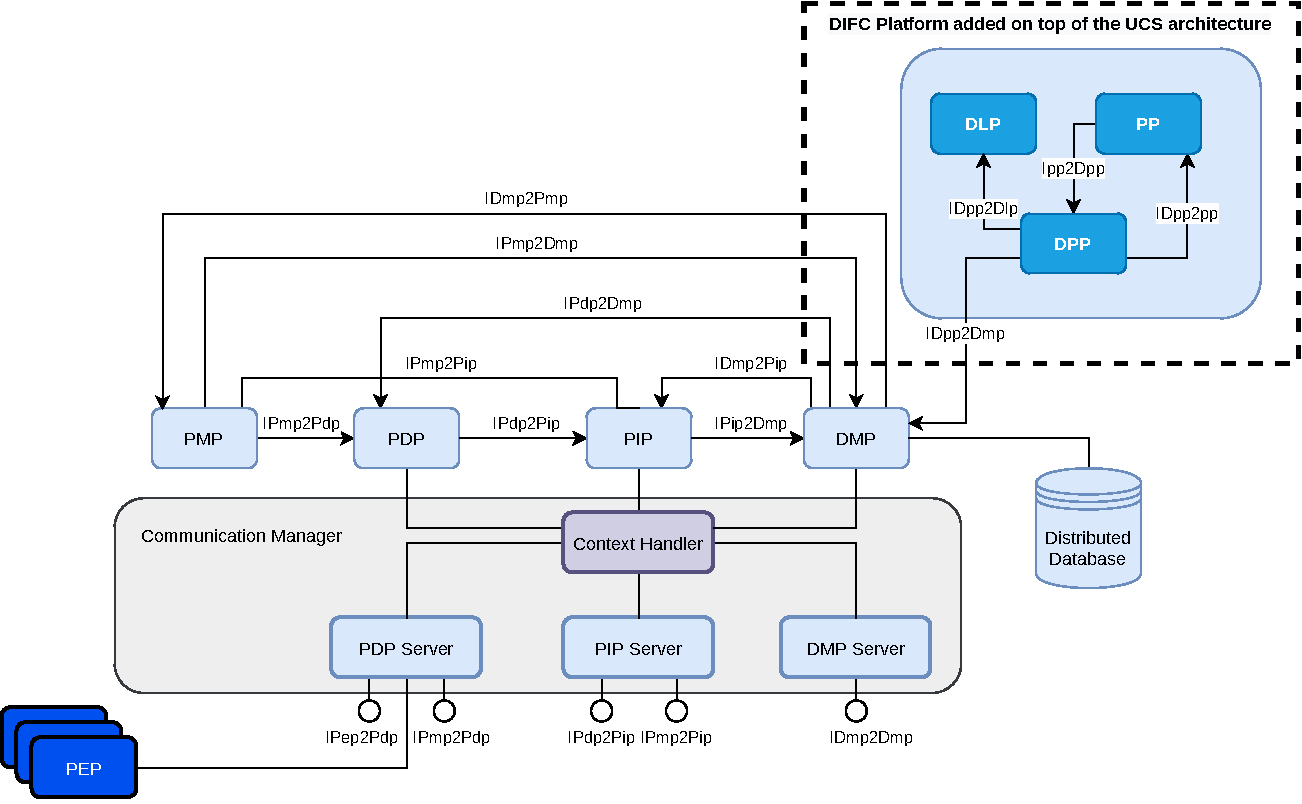
\includegraphics[width=\columnwidth]{Images/Kelbert_architecture_DIFC_enhanced.pdf}
% \caption{Architecture of the usage control system \cite{Kelbert2018}, with the DIFC platform for policy labeling as a contribution.}
% \label{F_Kelbert_architecture_DIFC_enhanced}

% \end{figure}
% This processing is often provided by a dedicated instance, called the DIFC platform \cite{Lu2022} or DIFC platform \cite{Schultz2013}. There are different ways to fulfill these tasks: either use already existing components, e.g., the PDP, or introduce new dedicated components to manage DIFC aspects. Since DIFC policies differ from usage control policies, it is better to introduce dedicated components to handle DIFC aspects.

% For distribution purposes, DIFC platform components are added as a novelty to the existing architecture, and interact only with the DMP to distribute the policies to other individual systems $\mathcal{Y}$ or system set $Y$. The DIFC platform is responsible for pre-processing (DPre), privilege extraction (PP) and data labeling (LD). Each operation has a dedicated component, as depicted in Figure~\ref{F_Kelbert_architecture_DIFC_enhanced}.

 \begin{figure}[t]
 \centering
 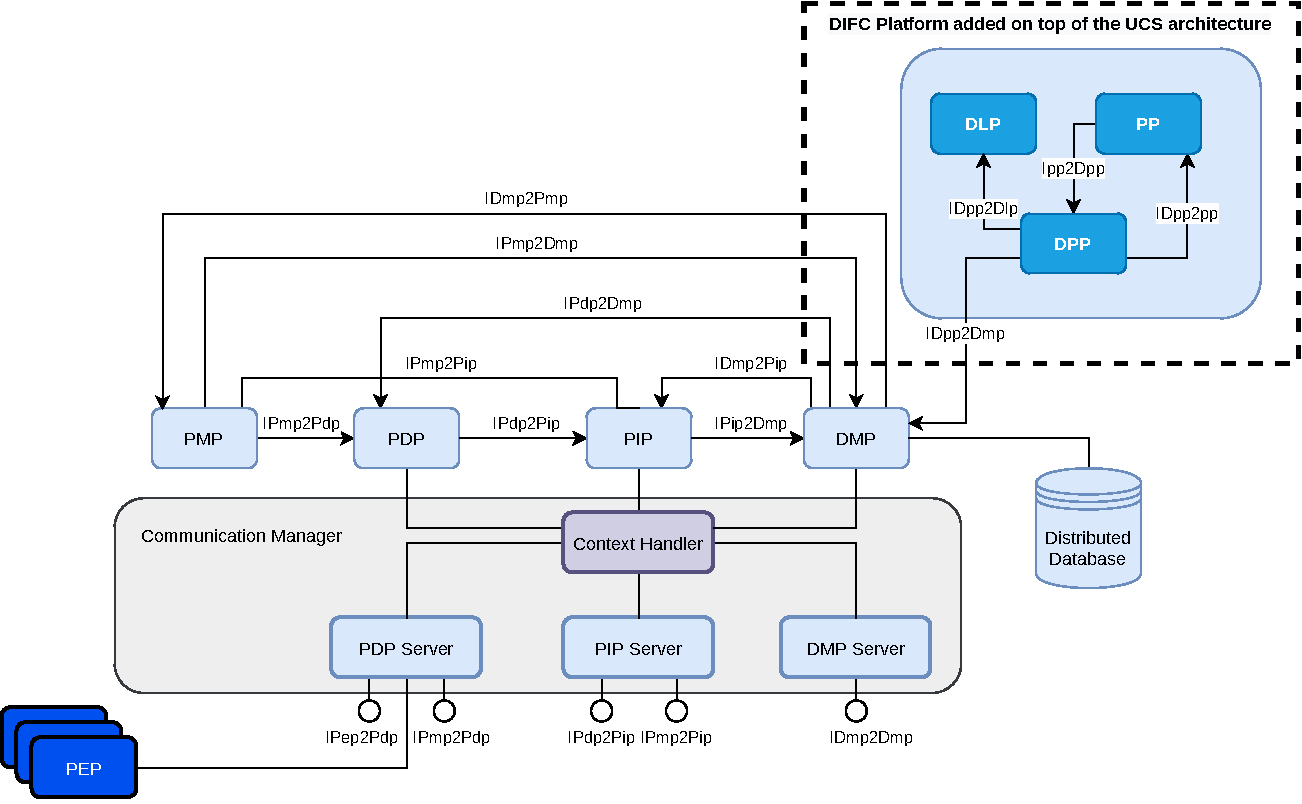
\includegraphics[width=\columnwidth]{Images/Kelbert_architecture_DIFC_enhanced.pdf}
 \caption{Architecture of the usage control system \cite{Kelbert2018}, with the DIFC platform for policy labeling as a contribution.}
\label{F_Kelbert_architecture_DIFC_enhanced}
\end{figure}

\textbf{DIFC interfaces.} As part of the contribution, the introduction of DIFC components requires to add four new interfaces (represented in Figure \ref{F_Kelbert_architecture_DIFC_enhanced}):
\begin{enumerate}
    \item \texttt{IDPP2DLP} is an interface implemented so that the data can be labeled by the data labeling point (DLP) if the component DPre detects that it has not been labeled yet;
    \item \texttt{IPP2DPP} is needed to answer a request from the data processing point (DPP) and to notify it with updates of privileges;
    \item \texttt{IDPP2PP} is an interface that enables the data pre-processing point (DPP) to fetch the required privileges from the dedicated privilege point; 
    \item \texttt{IDPP2DMP} provide methods so that the DIFC policies are propagated to all individual systems.
\end{enumerate}
%\section{Model checking}
%\label{S_model_checking}

%To ensure the correctness of the proposed system's design, we rely on model checking using \emph{TLC}, introduced in Section \ref{ss_background_tla}. Model checking is used in formal verification for early detection of errors or potential issues in a system design or specification, for an exhaustive exploration of all system states and behaviors and for design validation. The validation of the proposed function \emph{connected} is detailed in Section \ref{ss_validation}.

%\subsection{Background on TLA+ and TLC}
%\label{ss_background_tla}
%TLA+ is a general-purpose formal specification language based on
%the \emph{Temporal Logic of Actions} for specifying real-time properties
%\cite{Lamport1992}. It is designed for modeling and reasoning on concurrent and 
%distributed systems, which makes it appropriate to check our proposed model.

%\textbf{TLA+ model checker.} The TLA+ specifications corresponding to the proposed model's functions can be checked using model checking tools such as TLC (TLA+ Model Checker) or formally proven using theorem provers like TLAPS (TLA+ Proof System).

%\subsection{Validation of Connected function.}
%\label{ss_validation}

%\nathanael{Décrire ce qui est fait dans le code TLA+ pour l'exemple}
%\begin{figure}[t]
%    \centering
%     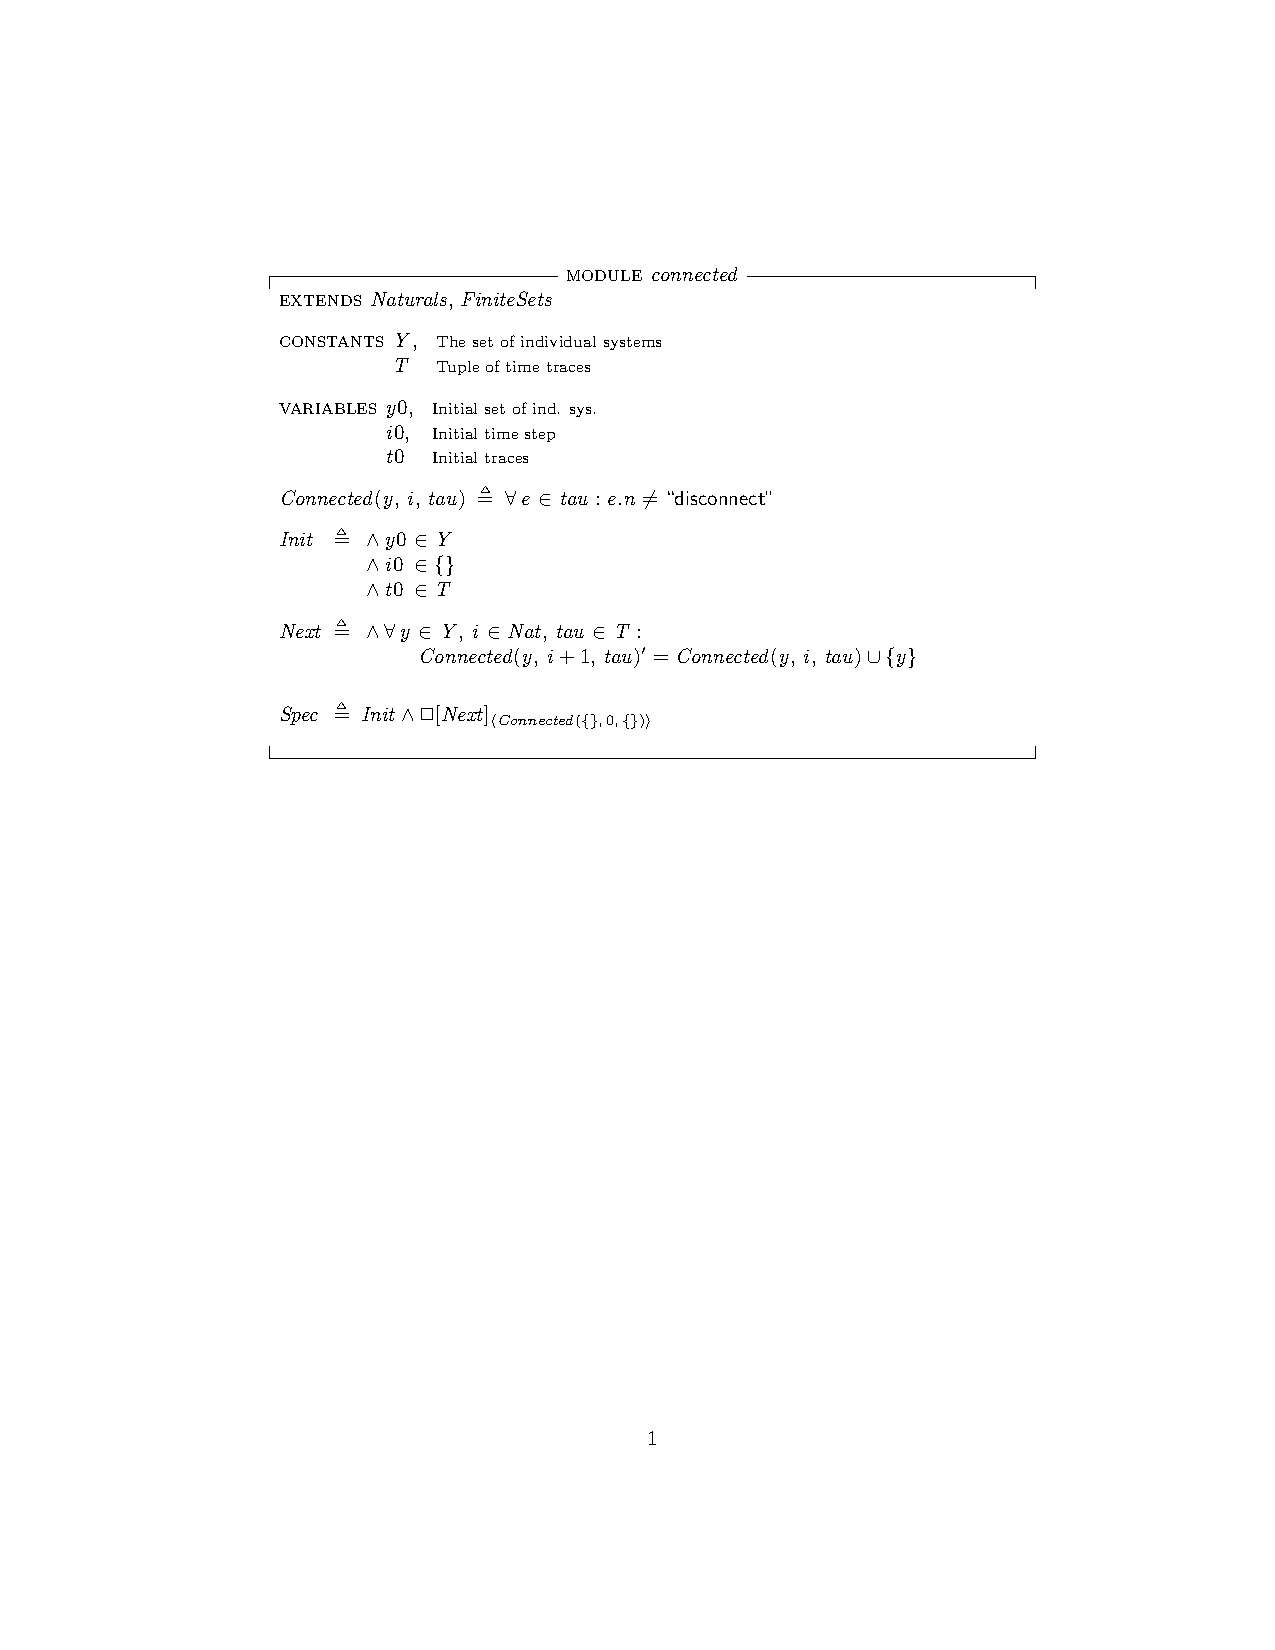
\includegraphics[trim=4.25cm 15cm 4cm 4cm, clip=true, width=\textwidth]{Images/connected.pdf}
%    \caption{Specification of connected function in TLA+}
%    \label{F_connected_TLA+}
%    \end{figure}
 
%\subsection{Validation of Conflict function.}

\section{Conclusion}
\label{S_conclusion_formalism}

In this chapter, we propose an extended usage control model for distributed systems, 
by introducing elements of decentralized information flow control (DIFC) into the state-of-the-art formalism~\cite{Kelbert2018}. 
The extension of the former modeling is justified by the need to consider all the aspects of the distribution, including 
the user-side policy definition, as well as specificities of IoT networks that require a more sophisticated 
distributed system modeling. Recent advances in DIFC, based on evolving coding practices \cite{Liu2022}, make DIFC usable 
and justify its consideration in distributed system modeling.
Although this formalism enables the addition of external specification, using the dedicated \underline{evalExt} operator, 
we state that DIFC actually requires dedicated components and functions. As a consequence, we extend the existing usage control architecture 
adding a privilege point (PP), a data pre-processing component (DPre) and a last component dedicated to data labeling (DL). Interfaces 
are also considered to enable cross-component communication. Additionally, 
we define new functions to identify the relevant parts of the distributed system. The main function considered, \emph{conflict},
detects individual systems $\mathcal{Y}$ (cf. Section \ref{ss_distributed_system_model}) of the distributed system where the
security policy on the data and their storage location are conflicting.

